% Chapter 2

\chapter{Literature Review} % Main chapter title

\label{Chapter2} % For referencing the chapter elsewhere, use \ref{Chapter1}

%----------------------------------------------------------------------------------------

% Define some commands to keep the formatting separated from the content

%----------------------------------------------------------------------------------------

\section{Cellular Automata and Game of Life}
Cellular Automata can be modelled in a number of dimensions including anything from one, two, three, four, or more dimensions.\citep{adamatzky2010game} In this project the focus will be on the two dimensional approach using a \textsl{n}-dimensional lattice (will be referred to as a grid). The grid can be of infinite size, however will be limited to a finite space i.e. a predetermined set of cells superimposed over a map of an informal settlement.\\\\
An individual square in the grid (which will be referred to as a cell) can have upto eight neighbours. This is shown in the diagram below.
\begin{figure}[H]
\centering
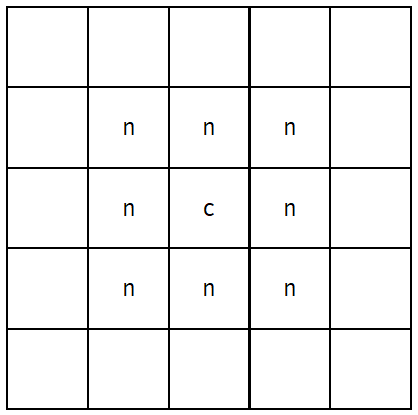
\includegraphics[scale=0.5]{Figures/cell.png}
\caption{A cell 'c' and its neighbours 'n'}
\label{fig:cell}
\begin{center}
Source: Own Creation (2021)
\end{center}
\end{figure}
A cell can have two discrete states for any given discrete time unit (referred to as generation). These states can be 'alive' or 'dead'. A cell is shown to be alive by having it \textsl{shaded} and if it is dead it is left blank.\citep{adamatzky2010game} This is shown in the figure below.
\begin{figure}[H]
\centering
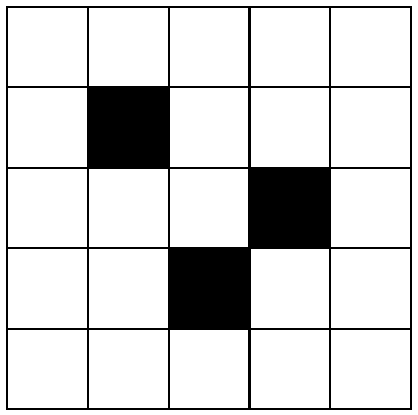
\includegraphics[scale=0.5]{Figures/shaded.png}
\caption{A grid showing alive and dead cells}
\begin{center}
Source: Own Creation (2021)
\end{center}
\end{figure}
As shown in Figure \ref{fig:cell} a cell can have either lateral or diagonal neighbours. The rules of \textsl{Life} were discussed briefly above in Section \ref{sec:prob}. A graphical representation of these is shown below.
\begin{figure}[H]
\centering
\begin{subfigure}{.5\textwidth}
  \centering
  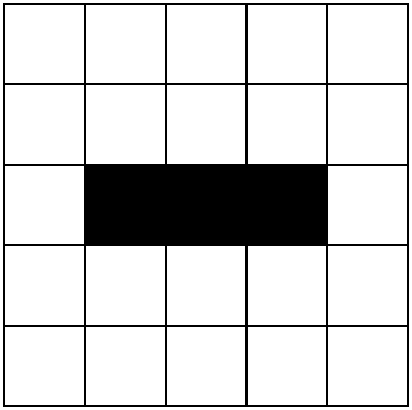
\includegraphics[width=.4\linewidth]{Figures/blink1.png}
  \caption{Generation $t = 0$}
\end{subfigure}%
\begin{subfigure}{.5\textwidth}
  \centering
  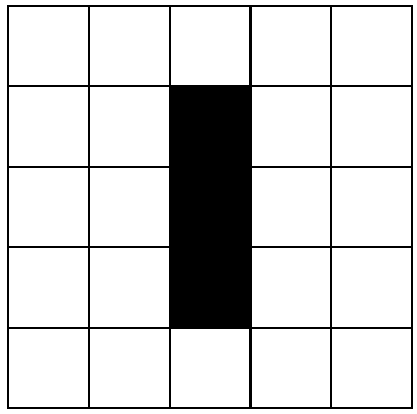
\includegraphics[width=.4\linewidth]{Figures/blink2.png}
  \caption{Generation $t = 1$}
\end{subfigure}
\caption{A simple 2 generation iteration of \textsl{Life}}
\begin{center}
Source: Own Creation (2021)
\end{center}
\end{figure}
Another slightly more advanced setup of \textsl{Life} is shown below.
\begin{figure}[H]
\centering
\begin{subfigure}{.5\textwidth}
  \centering
  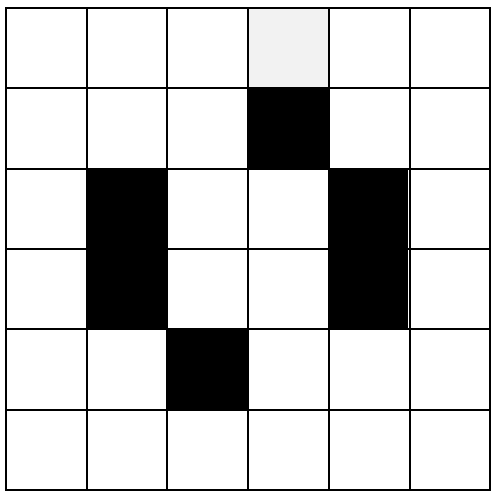
\includegraphics[width=.4\linewidth]{Figures/toad1.png}
  \caption{Generation $t = 0$}
\end{subfigure}%
\begin{subfigure}{.5\textwidth}
  \centering
  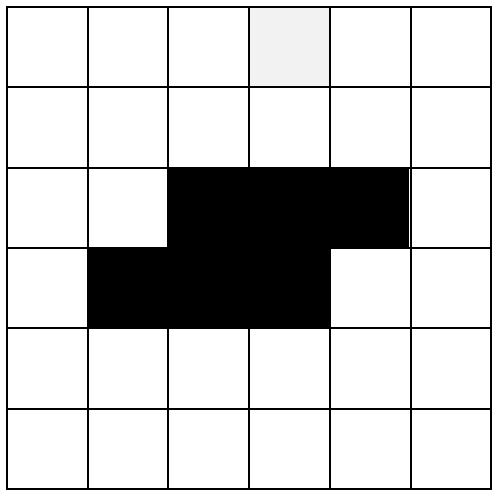
\includegraphics[width=.4\linewidth]{Figures/toad2.png}
  \caption{Generation $t = 1$}
\end{subfigure}
\caption{An advanced 2 generation iteration of \textsl{Life}}
\begin{center}
Source: Own Creation (2021)
\end{center}
\end{figure}
In a seminal paper by Stephen Wolfram, four classes of CA were proposed according to their behaviour given an initial random condition .\citep{Wolfram1984} These four classes are as follows:
\begin{itemize}
\item Class 1 - After a finite number of generations a unique homogeneous state is reached i.e. all cells become the same eventually.
\item Class 2 - Simple structures are generated which are either periodic, or stable (also called persistent).
\item Class 3 - An aperiodic (or chaotic) patterns emerge which carry on indefinitely.
\item Class 4 - Capable of universal computations i.e. can exhibit complex behaviour. 
\end{itemize}
Due to the nature of the rules of \textsl{Life} certain patterns emerge. This is thanks to the cycles of repeated stated which evolve over certain number of generations. These patterns include still-lifes, period two (or \textsl{blinkers}), gliders, oscillators, glider guns, and puffer trains.\citep{adamatzky2010game}
\\\\
The applications of CA and, or \textsl{Life} have sparked a number of research papers in fields such as physics, music, complexity, and computation. \\
Examples in physics include, interaction between a complex system and electromagnetic radiation \citep{conti}, an implementation of \textsl{Life} with quantum features.\citep{quantum}\\
Implementations in music include the development of CAMUS (\textbf{C}ellular \textbf{A}utomata \textbf{Mus}ic).\citep{music}\\
In the fields of complexity, and computation a vast array of work has been done therefore a few examples include; Universal Computer-Constructor in CA \citep{gou}, and creation of a Turing Machine in \textsl{Life}.\citep{ren}
\section{Informal settlements}
Informal settlements are housing dwellings that are part of urban districts or neighbourhoods that arise and develop without oversight or control from the state. They are synonymous with 'slums' or 'squatters', though are not the same. They form an integral element of urban sustainability whereby developing cities can not develop without them. The connotations with 'informal', 'slums', and 'squatter' have always been seen in a negative light. This is not seen as beneficial as the growth of urbanisation is highly intertwined with informal settlements.\citep{dovey2011forms}\\
Across the globe informal settlements are known colloquially by their own variety of terms. \citep{un} In this project the umbrella term informal settlement will be utilised.\\
The process of informal settlements growth can be grouped into three categories namely;\citep{dovey2011forms}
\begin{itemize}
\item \textsl{settling} - simply settling down on what is usually unclaimed land
\item \textsl{inserting} - usually into urban areas that are abandoned, or uninhabited
\item \textsl{attaching} - informal settlements that grow out of existing urban settlements
\end{itemize}
In morphological terms, informal settlements can be classified into eight different types. This refers to the urban conditions rather that the process mentioned above, however it is not to say that the two are mutually exclusive. The types are not mutually exclusive from each other either. The types are as follows:\citep{dovey2011forms}
\begin{itemize}
\item Districts - 
\item Waterfronts - 
\item Escarpments - 
\item Easements - 
\item Sidewalks - 
\item Adherences -
\item Backstages -
\item Enclosures - 
\end{itemize}